\section{Langkah-Langkah Percobaan}
Di percobaan Routing Dan Manajemen IPV6, kita menggunakan 2 laptop dan 2 router mikrotik, serta software winbox. Pertama, dihubungkanlah semua device menggunakan kabel lan (pc1-router1-router2-pc2). Router pun direset. Lalu set ip address tiap laptop, serta konfigurasi untuk routing dinamis. Setelah itu dilakukan test ping untuk menghubungkan antara kedua laptop. Setelah routing statis berhasil dikonfigurasikan lah routing dinamis, dan dilakukan uji ping lagi.

\section{Analisis Hasil Percobaan}
Di percobaan routing statis, ether1 router1 disetting ke 2001:db8:1::1/64 dan ether1 router2 disetting ke 2001:db8:1::2/64. Ether2 router1 menggunakan 2001:db8:a::1/64 dan ether2 router2 menggunakan 2001:db8:b::1/64. Selanjutnya, rute statis disetting, untuk router 1 tujuannya 2001:db8:b::/64 dan gatewaynya 2001:db8:1::2, sedangkan untuk router 2 tujuan 2001:db8:a::/64 dan gateway nya 2001:db8:1::1. Pada routing dinamis, setelah menyetting OSPFv3, routerID router 1 diset ke 1.1.1.1 dan routerID router 2 diset ke 2.2.2.2. Area ID di set ke 0.0.0.0. Percobaan ping berhasil di kedua percobaan.

\section{Hasil Tugas Modul}
\begin{enumerate}
	\item Terlampir
\end{enumerate}

\section{Kesimpulan}
Bahwa kita dapat mengonfigurasi IPV6 antar perangkat untuk memungkinkan mereka berkomunikasi, baik itu secara dinamis ataupun statis.

\section{Lampiran}
\subsection{Dokumentasi saat praktikum}
\begin{figure}
    \centering
    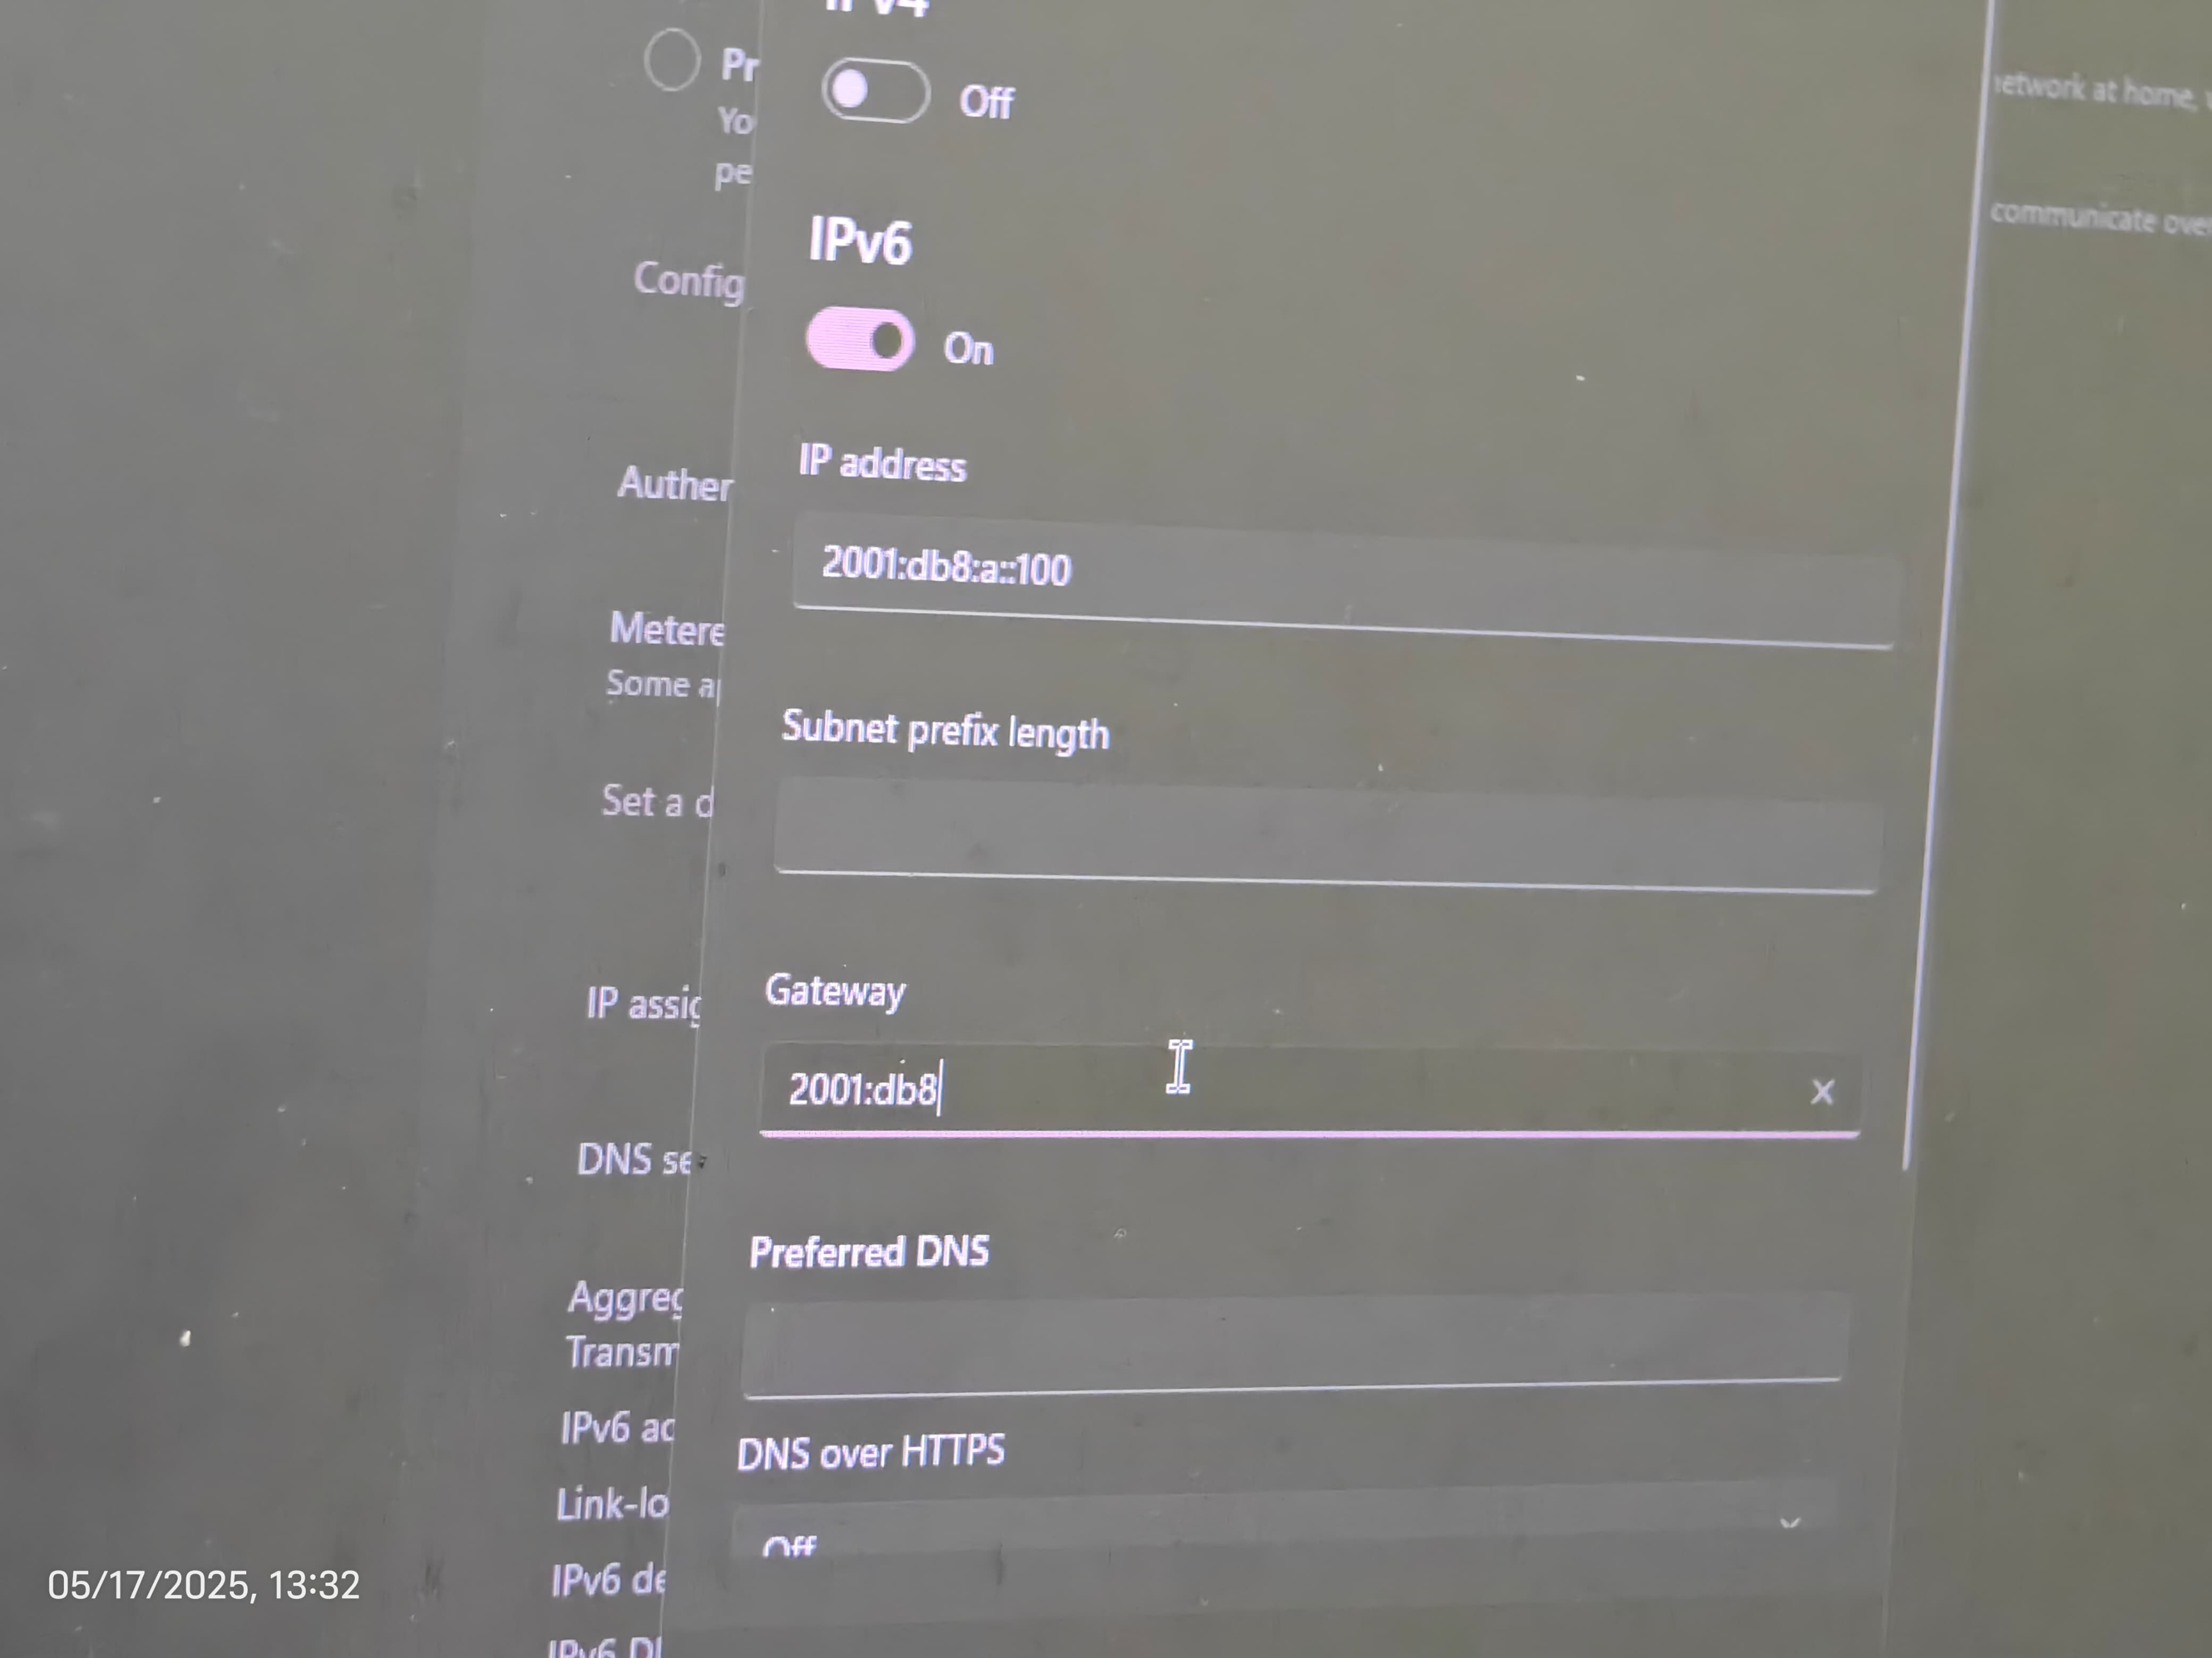
\includegraphics[width=0.5\linewidth]{Template Laporan Akhir/P1/img/WhatsApp Image 2025-05-17 at 14.44.31.jpeg}
    \caption{5.1 Setup router}
    \label{fig:enter-label}
\end{figure}
\begin{figure}
    \centering
    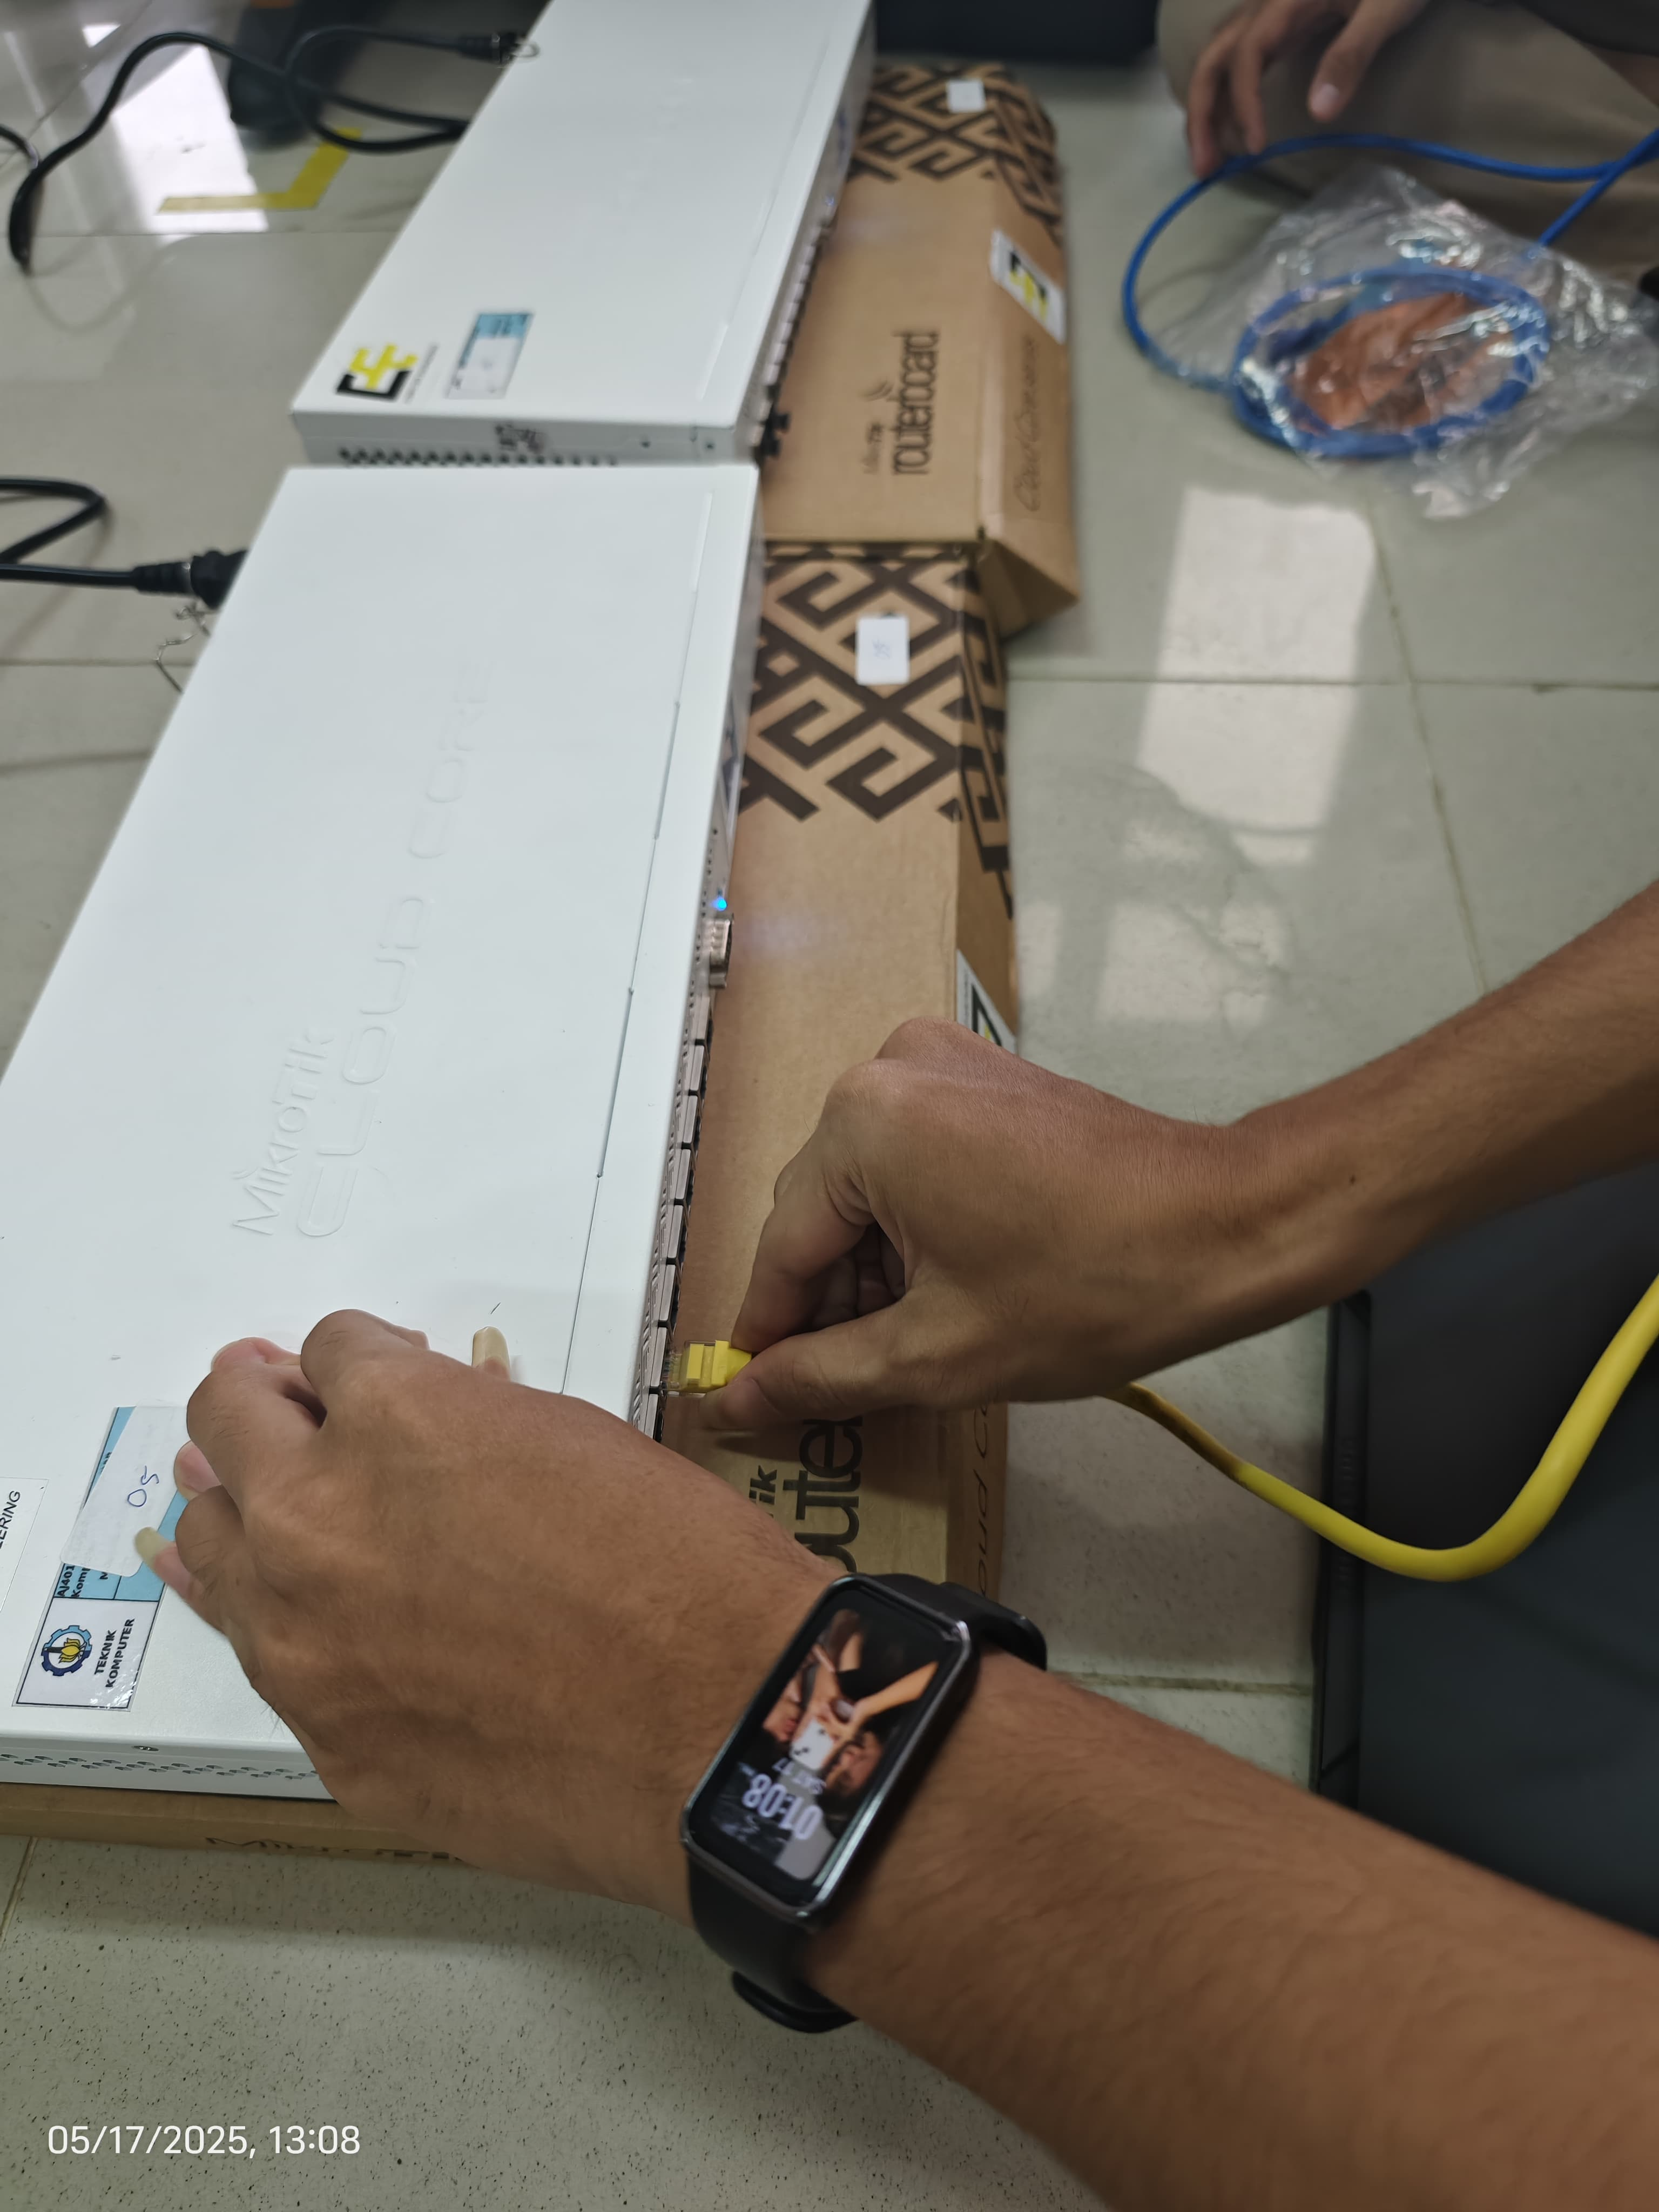
\includegraphics[width=0.5\linewidth]{Template Laporan Akhir/P1/img/WhatsApp Image 2025-05-17 at 14.44.39.jpeg}
    \caption{5.1 Config ipv6}
    \label{fig:enter-label}
\end{figure}
\begin{figure}
    \centering
    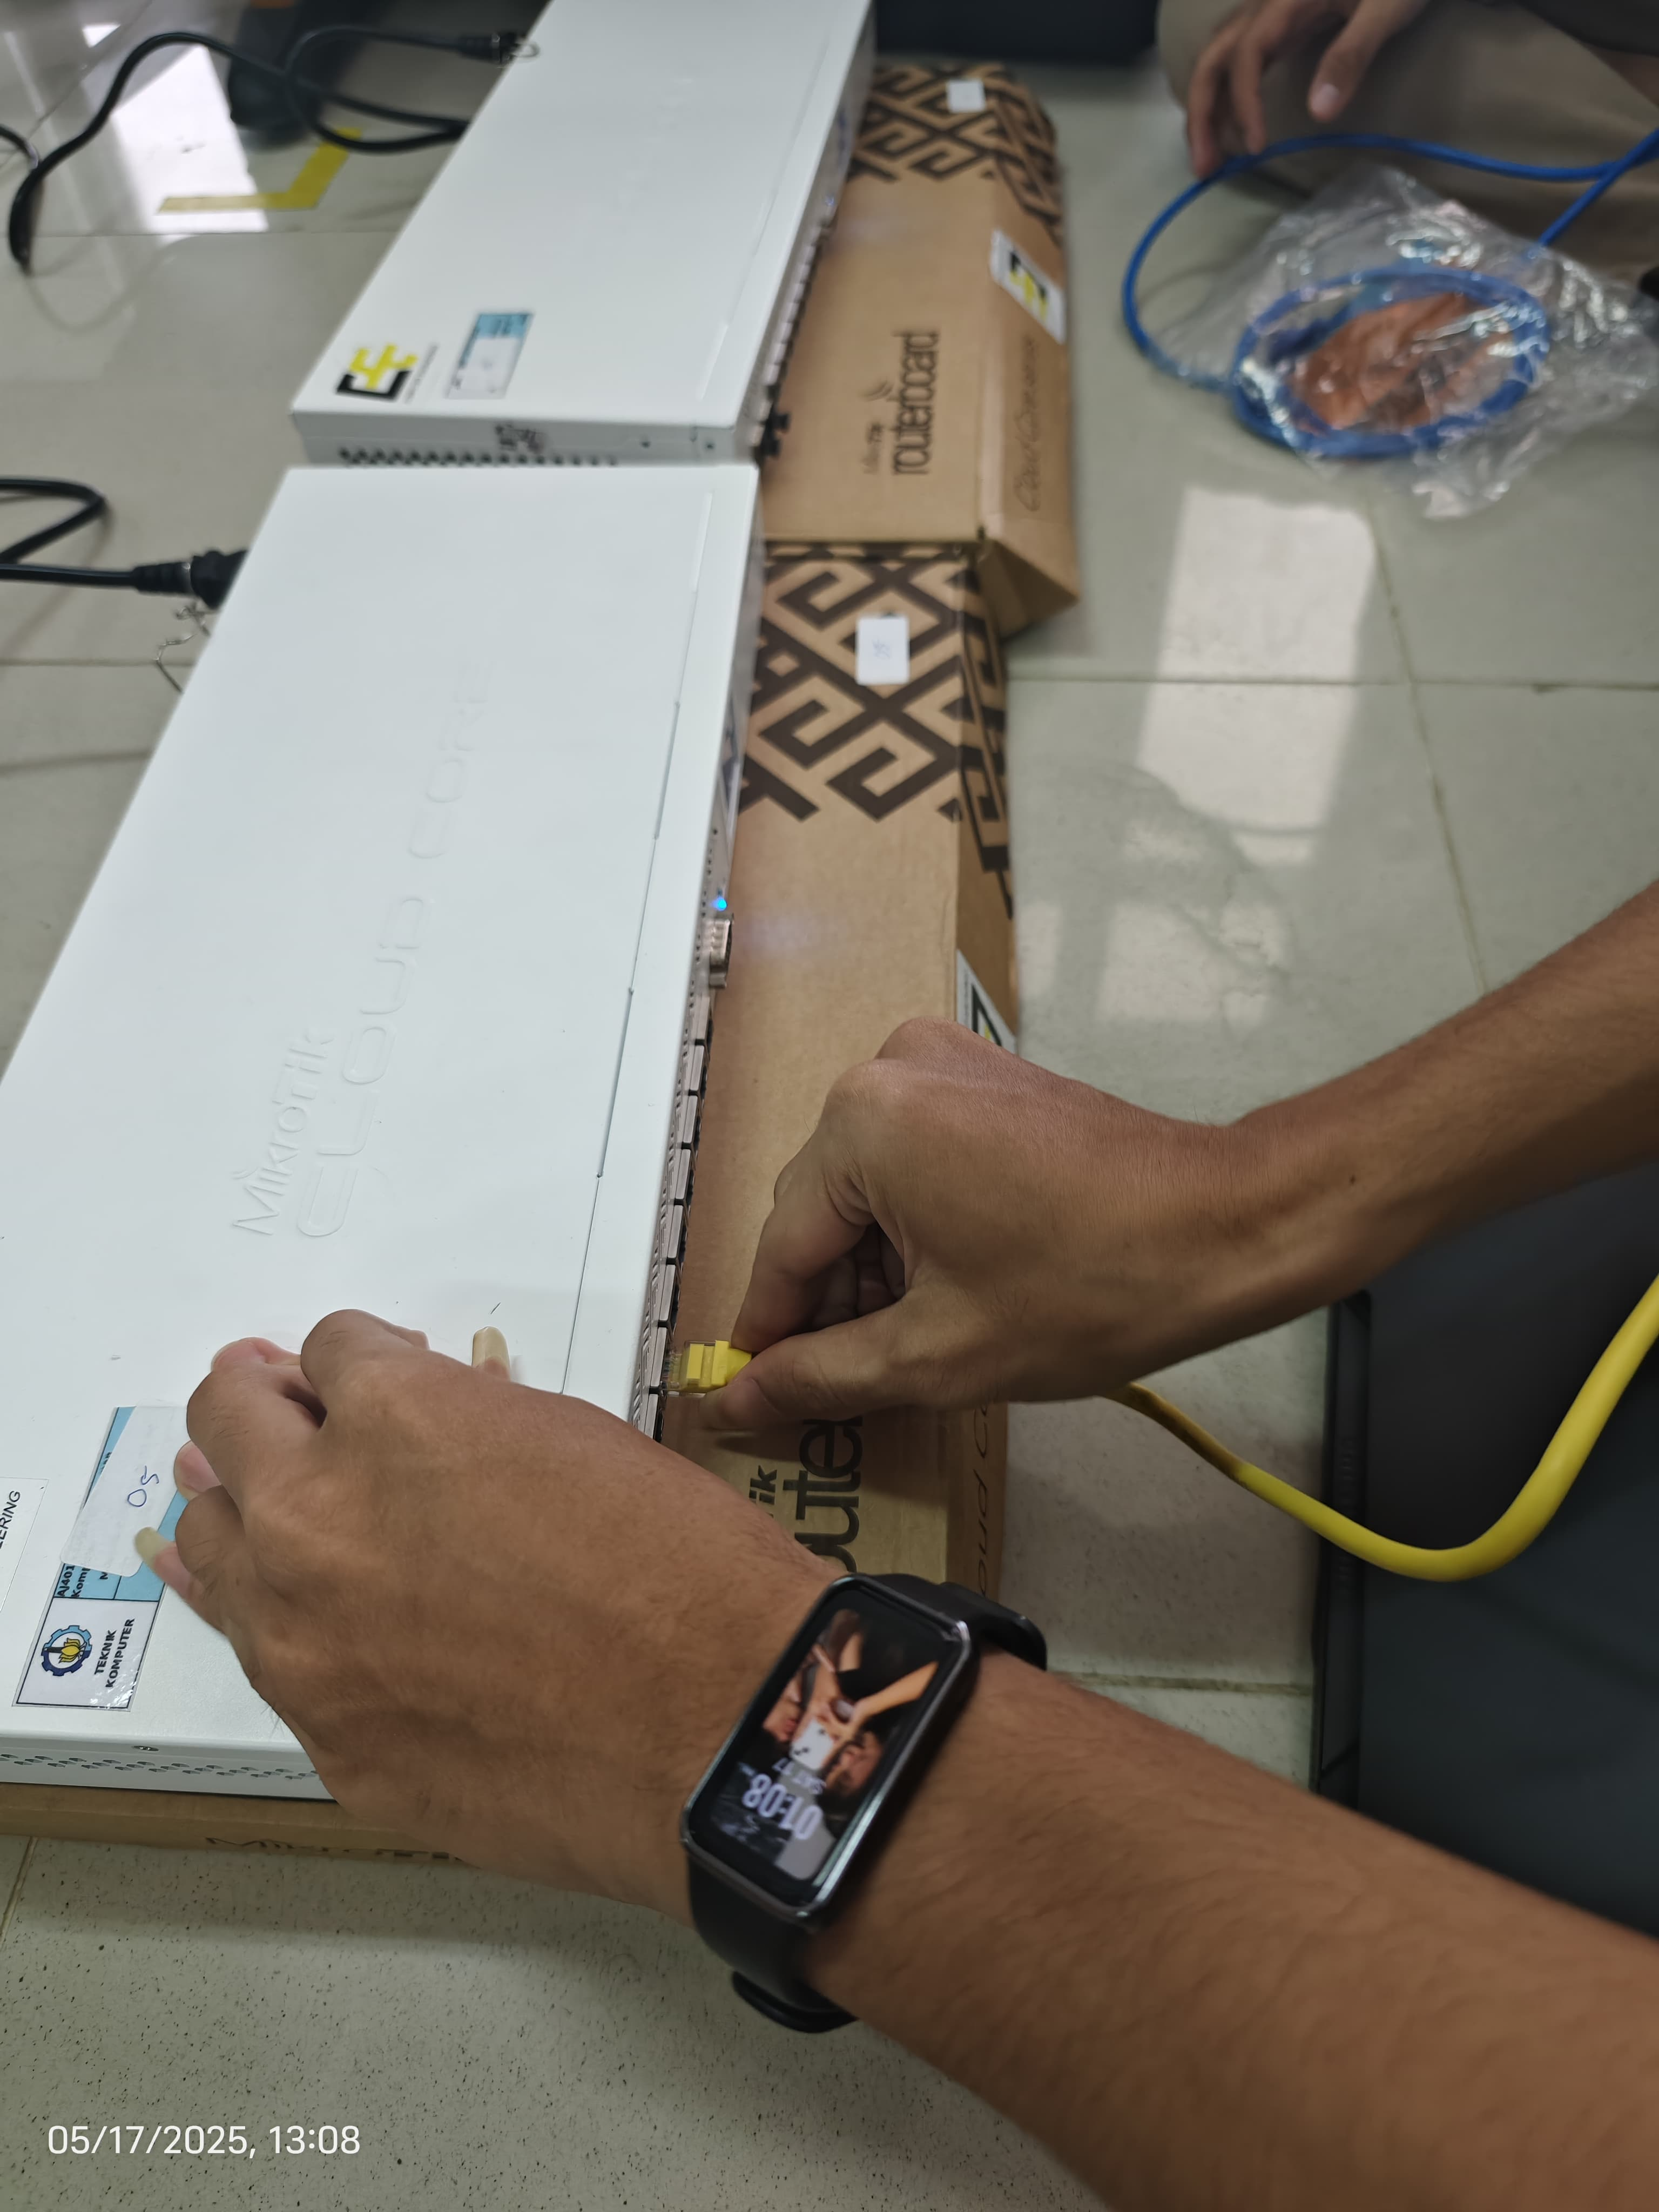
\includegraphics[width=0.5\linewidth]{Template Laporan Akhir/P1/img/WhatsApp Image 2025-05-17 at 14.44.39.jpeg}
    \caption{5.1 Ping statis berhasil}
    \label{fig:enter-label}
\end{figure}
\begin{figure}
    \centering
    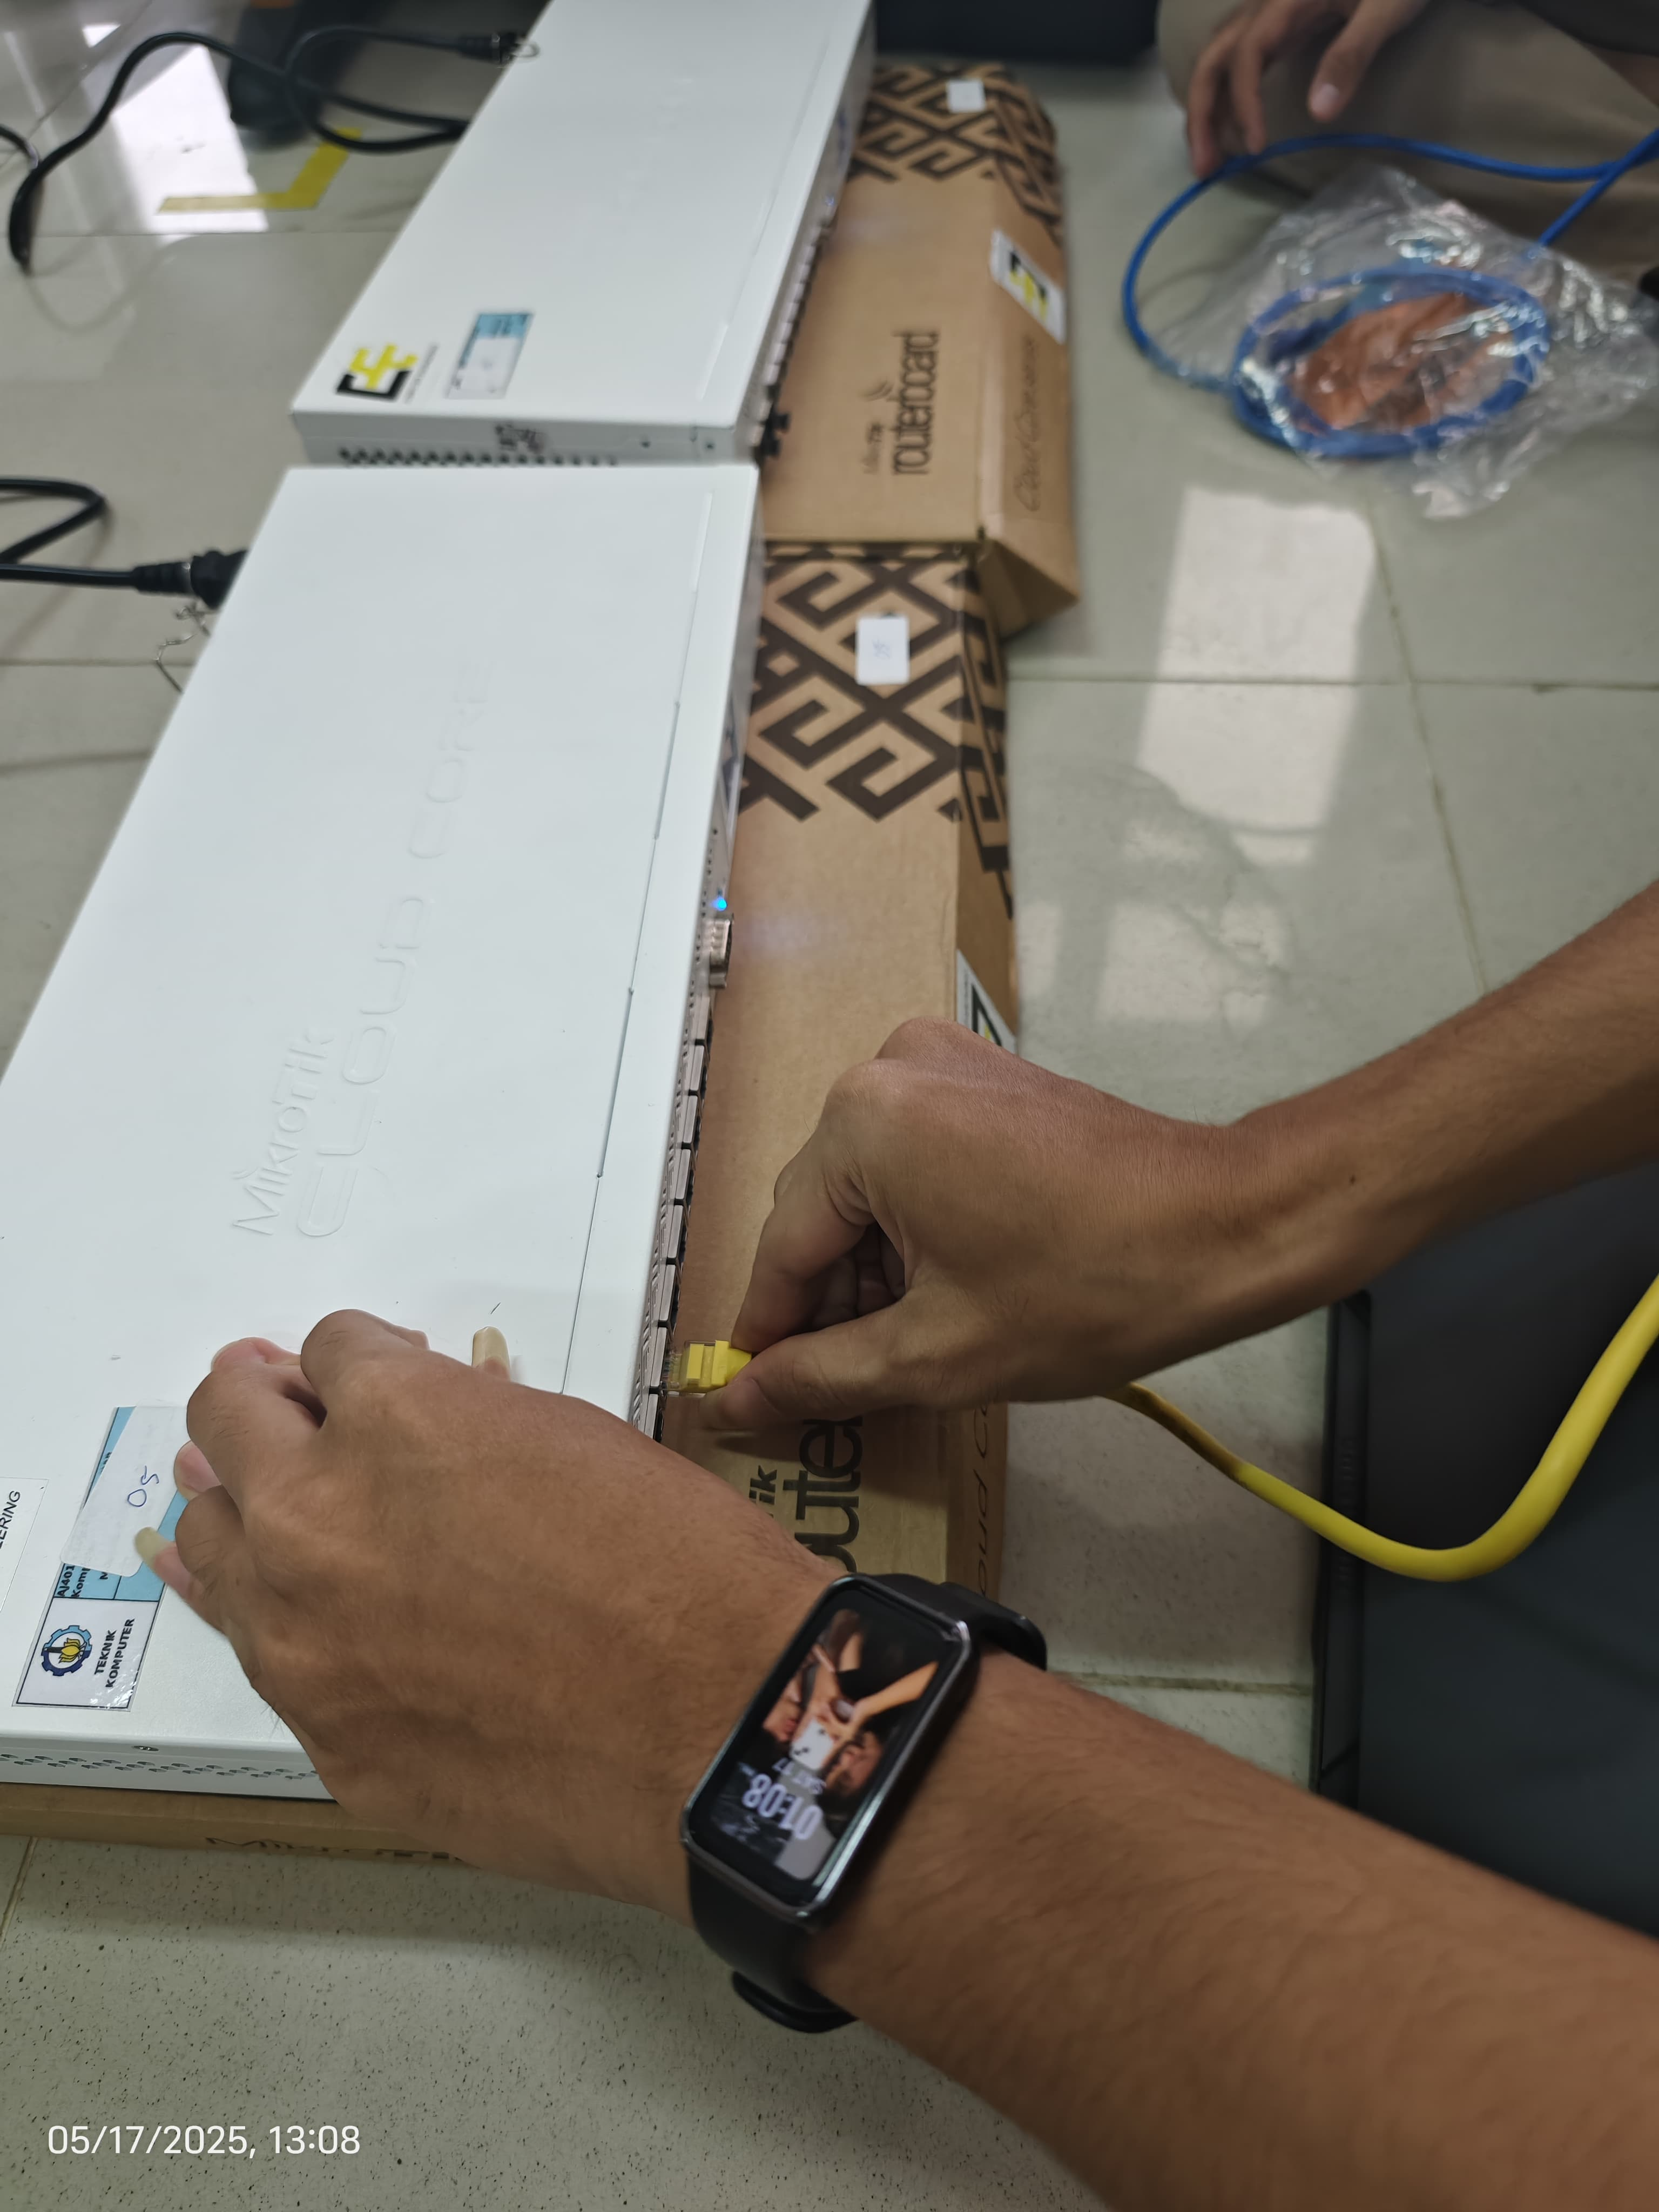
\includegraphics[width=0.5\linewidth]{Template Laporan Akhir/P1/img/WhatsApp Image 2025-05-17 at 14.44.39.jpeg}
    \caption{5.1 Ping dinamis berhasil}
    \label{fig:enter-label}
\end{figure}
\subsection{Lampiran tugas modul}
\begin{figure}
    \centering
    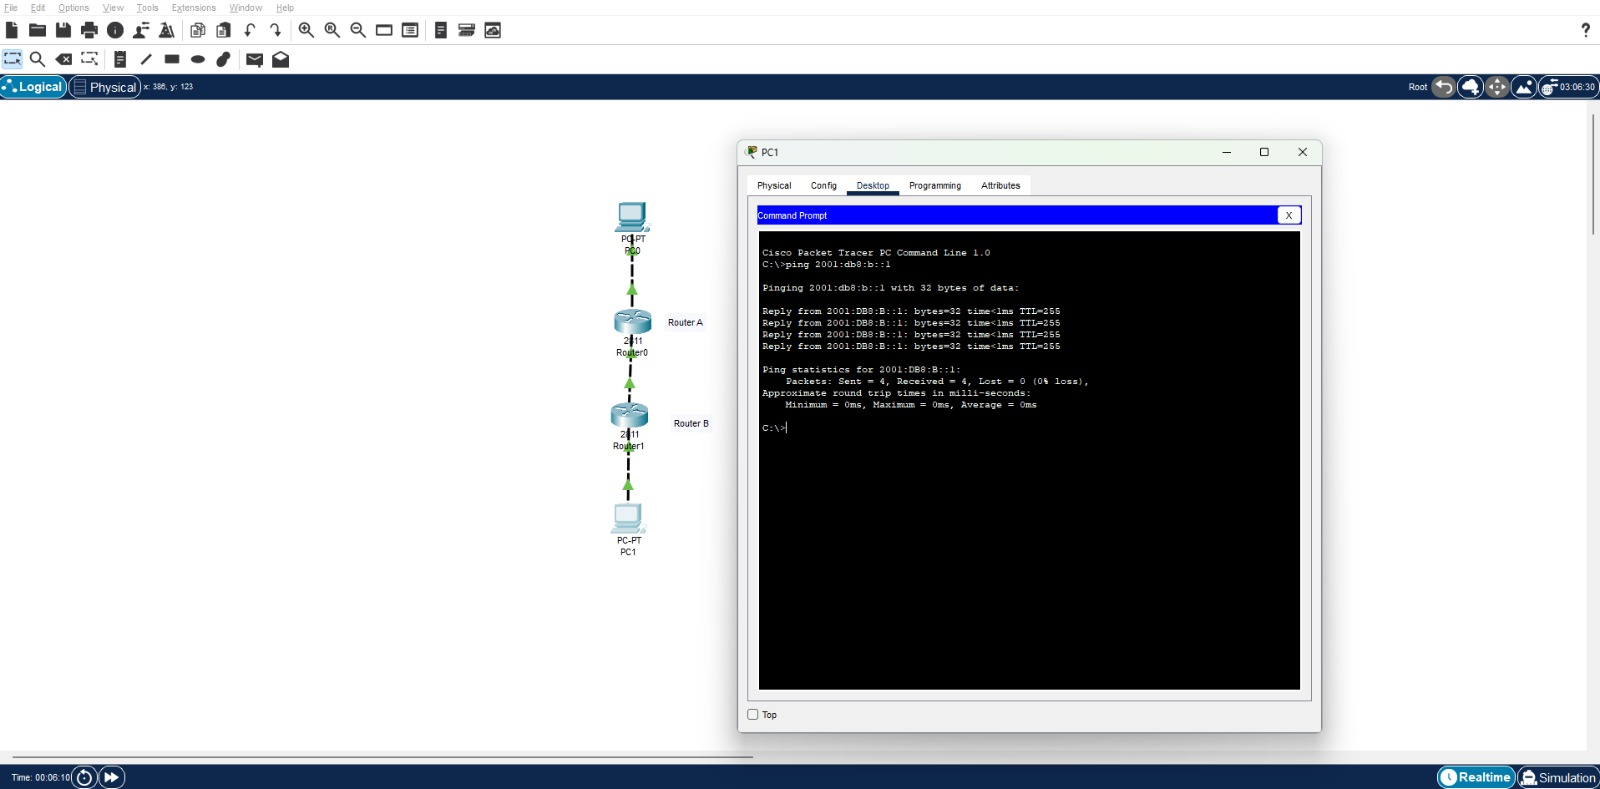
\includegraphics[width=0.5\linewidth]{Template Laporan Akhir/P1/img/WhatsApp Image 2025-05-26 at 20.13.24.jpeg}
    \caption{5.2 Statis: Ping PC1 ke PC2 berhasil}
    \label{fig:enter-label}
\end{figure}
\begin{figure}
    \centering
    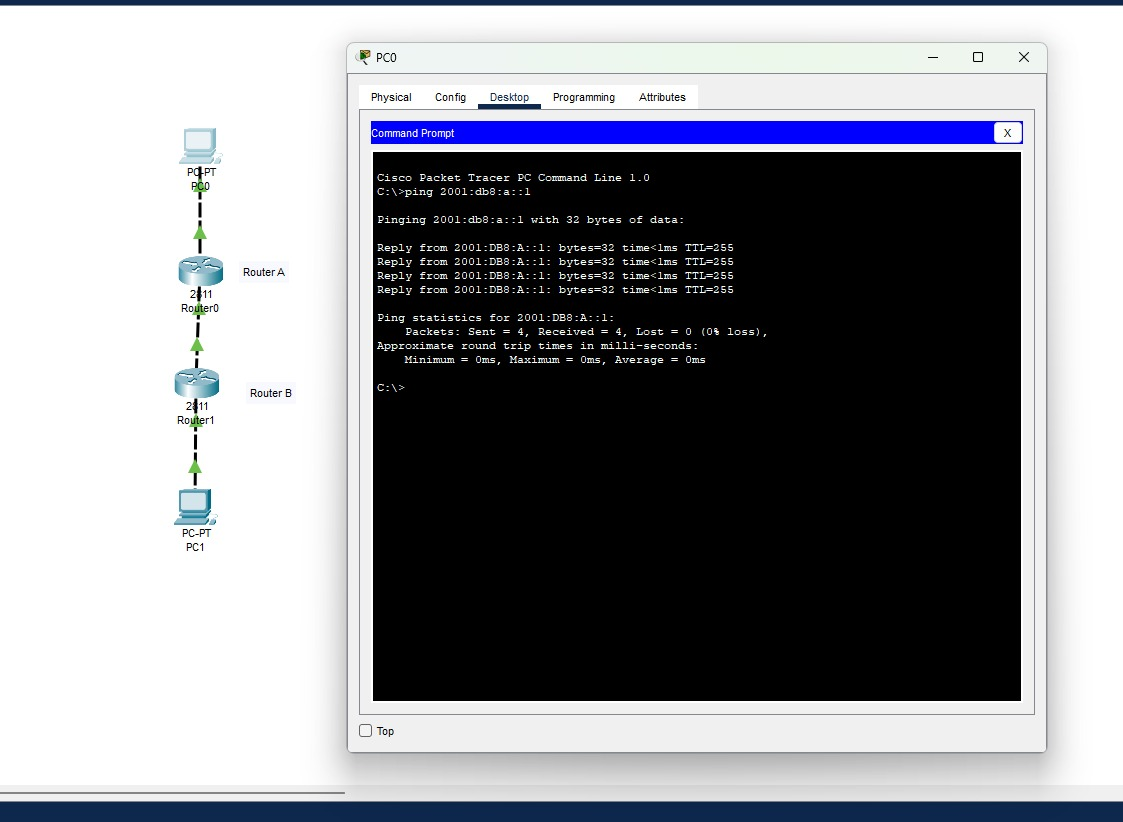
\includegraphics[width=0.5\linewidth]{Template Laporan Akhir/P1/img/WhatsApp Image 2025-05-26 at 20.16.09.jpeg}
    \caption{5.2 Statis: Ping PC2 ke PC1 berhasil}
    \label{fig:enter-label}
\end{figure}
\begin{figure}
    \centering
    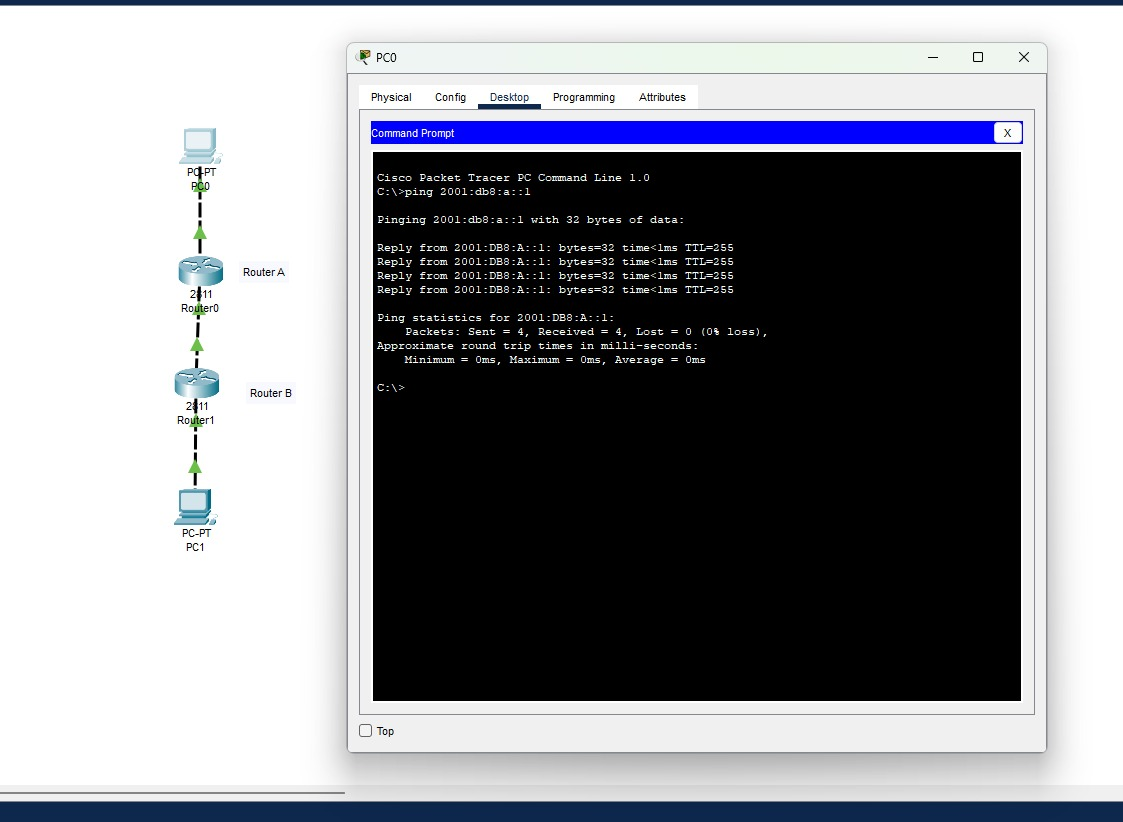
\includegraphics[width=0.5\linewidth]{Template Laporan Akhir/P1/img/WhatsApp Image 2025-05-26 at 20.16.09.jpeg}
    \caption{5.2 Dinamis: Ping PC2 ke PC1 berhasil}
    \label{fig:enter-label}
\end{figure}
\begin{figure}
    \centering
    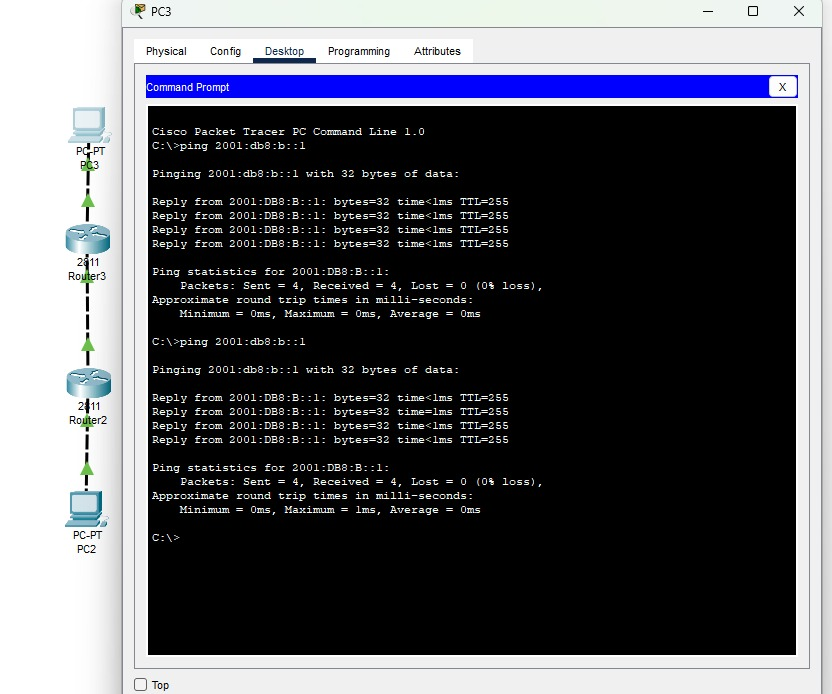
\includegraphics[width=0.5\linewidth]{Template Laporan Akhir/P1/img/WhatsApp Image 2025-05-26 at 20.41.39.jpeg}
    \caption{5.2 Dinamis: Ping PC1 ke PC2 berhasil}
    \label{fig:enter-label}
\end{figure}